\section{GNN Implementation}
\label{sec:4_6}

Four GNN architectures are implemented, sharing a common interface for fair comparison.

\begin{figure}[htbp]
    \centering
    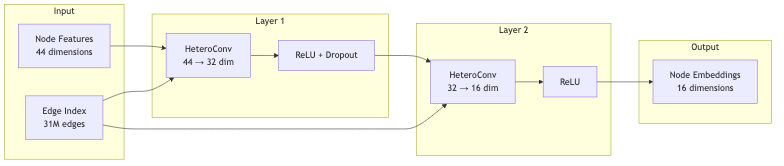
\includegraphics[width=\textwidth]{figures/fig_4_4_5_1.png}
    \caption{GNN Architecture: Input → Layers → Embeddings}
    \label{fig:4_4}
\end{figure}

\subsection{Model Architectures}
\label{sec:4_6_1}

\textbf{GraphSAGE Implementation:} The \texttt{GraphSAGEEncoder} uses PyTorch Geometric's \texttt{HeteroConv} wrapper to handle heterogeneous edge types. For each layer, the encoder creates separate \texttt{SAGEConv} modules (with mean aggregation) for each edge type (shares\_device, shares\_ip, shares\_email, shares\_phone, shares\_user), wrapping them in a \texttt{HeteroConv} layer with sum aggregation across edge types. The forward pass applies each convolutional layer sequentially, followed by ReLU activation and 0.3 dropout. The architecture supports configurable input channels (44 features), hidden channels (32), output channels (16), and number of layers (2). Complete PyTorch implementation is provided in Appendix~B.

\textbf{HGT Implementation:} Uses HeteroConv with HGTConv layers for multi-head attention on heterogeneous graphs.

\textbf{CARE-GNN Implementation:} Adds reinforcement learning-based neighbor selector using similarity measures (label-aware, feature-aware, relation-aware) to filter camouflaged connections.

\textbf{PC-GNN Implementation:} Implements label-balanced mini-batch sampling and confidence-based neighbor weighting for imbalanced fraud detection.

\subsection{Training Loop}
\label{sec:4_6_2}

Supervised training uses node classification with fraud labels. The training loop iterates for a fixed number of epochs (typically 30), processing mini-batches via PyTorch Geometric's \texttt{NeighborLoader}. For each batch: (1) gradients are zeroed, (2) the model performs forward propagation on the batch's node features and edge indices, (3) binary cross-entropy loss with logits is computed on training nodes only (using train\_mask), with pos\_weight=11.0 to handle class imbalance, (4) gradients are computed via backpropagation, and (5) the optimizer updates model parameters. Complete training implementation including validation and early stopping is provided in Appendix~B.
